    
\setcounter{chapter}{1}
\setcounter{subsection}{0}
\chapter{Multiplicando a fração da unidade }


\noindent\begin{tabular}{cc}
 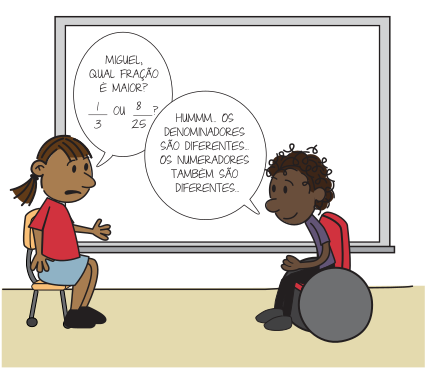
\includegraphics[width=.45\textwidth, keepaspectratio]{../../livro/media/cap2/secoes/pngs_licao_02/quadrinho_01.png}   & 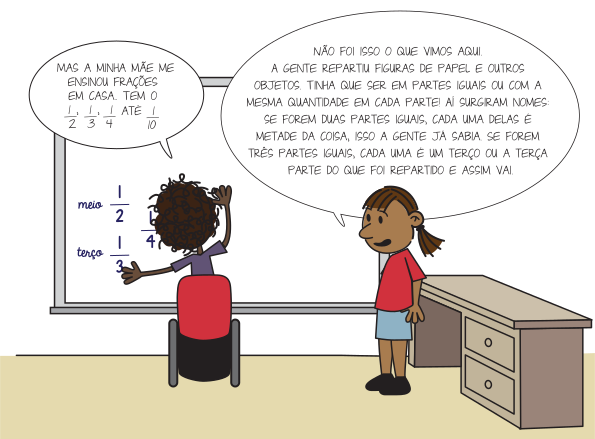
\includegraphics[width=.45\textwidth, keepaspectratio]{../../livro/media/cap2/secoes/pngs_licao_02/quadrinho_02.png}   \\
 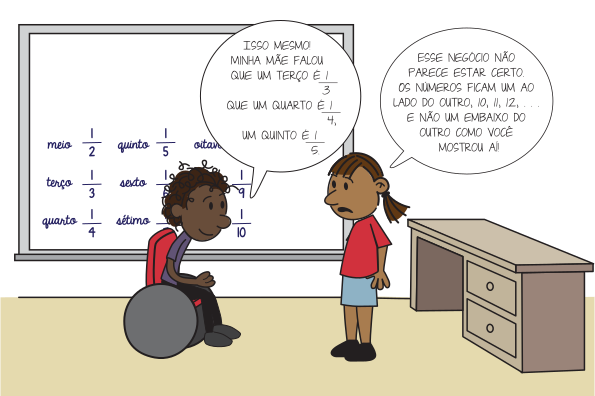
\includegraphics[width=.45\textwidth, keepaspectratio]{../../livro/media/cap2/secoes/pngs_licao_02/quadrinho_03.png} & 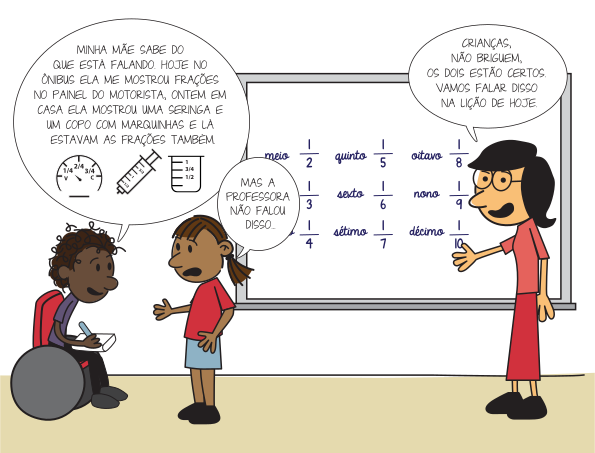
\includegraphics[width=.45\textwidth, keepaspectratio]{../../livro/media/cap2/secoes/pngs_licao_02/quadrinho_04.png}     
\end{tabular}


  
    

    
\section{EXPLORANDO O ASSUNTO }

\subsection{Atividade}

O pai de Ana, Beatriz e Clara trouxe duas barras de chocolate para serem repartidas entre elas.

\begin{center}

\begin{tikzpicture}[scale=0.9]
\draw[fill=Sepia] (0,0) rectangle (60,20);
\end{tikzpicture}
\end{center}

Ana propôs que cada barra fosse dividida em três partes iguais e que cada irmã ficasse com duas dessas partes.


\begin{center}
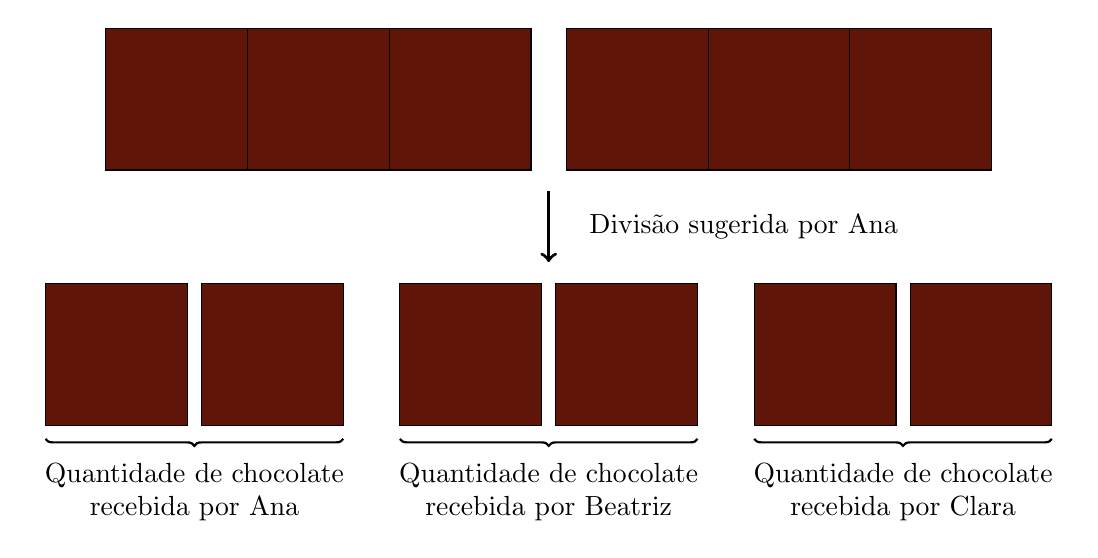
\begin{tikzpicture}[x=1mm,y=1mm,scale=0.9]
\draw[fill=Sepia] (0,0) rectangle (60,20);
\draw (20,0) -- (20,20);
\draw (40,0) -- (40,20);

\draw[fill=Sepia, shift={(65,0)}] (0,0) rectangle (60,20);
\draw[shift={(65,0)}] (20,0) -- (20,20);
\draw[shift={(65,0)}] (40,0) -- (40,20);

\draw[very thick, shift={(62.5,-3)}, ->] (0,0) -- (0,-10);  
\node at (90,-8) {Divisão sugerida por Ana};

\draw[fill=Sepia, shift={(-8.5,-36)}] (0,0) rectangle (20,20);
\draw[fill=Sepia, shift={(13.5,-36)}] (0,0) rectangle (20,20);

\draw[fill=Sepia, shift={(41.5,-36)}] (0,0) rectangle (20,20);
\draw[fill=Sepia, shift={(63.5,-36)}] (0,0) rectangle (20,20);

\draw[fill=Sepia, shift={(63.5 + 28,-36)}] (0,0) rectangle (20,20);
\draw[fill=Sepia, shift={(63.5 + 50,-36)}] (0,0) rectangle (20,20);

\draw [thick, decoration={brace,mirror,raise=5}, decorate] (-8.5,-36) -- (33.5,-36) 
node [pos=0.5,anchor=north,yshift=-10] {\parbox[b]{40mm}{\centering Quantidade de chocolate recebida por Ana}}; 

\draw [thick, decoration={brace,mirror,raise=5}, decorate] (41.5,-36) -- (83.5,-36) 
node [pos=0.5,anchor=north,yshift=-10] {\parbox[b]{40mm}{\centering Quantidade de chocolate recebida por Beatriz}}; 

\draw [thick, decoration={brace,mirror,raise=5}, decorate] (63.5+28,-36) -- (63.5+70,-36) 
node [pos=0.5,anchor=north,yshift=-10] {\parbox[b]{40mm}{\centering Quantidade de chocolate recebida por Clara}}; 

\end{tikzpicture}
\end{center}

\begin{enumerate}[a)] %s
  \item Na divisão de cada uma das barras de chocolate em três partes iguais, cada parte é que fração de uma barra de chocolate?
  \item Você concorda com a divisão que Ana sugeriu? Explique. 
  \item Com essa divisão, as três irmãs receberiam a mesma quantidade de chocolate? 
  \item Na divisão proposta por Ana, como você nomearia, usando uma fração de uma barra de chocolate, a quantidade de chocolate que cada irmã receberia? 
\end{enumerate}
  
Ana não quer o chocolate e decidiu dar a quantidade de chocolate que recebeu na divisão das barras para as suas irmãs.

\begin{enumerate}[e)]
\item Se Ana desse metade da quantidade de chocolate que recebeu para cada uma de suas irmãs, que quantidade de chocolate Beatriz e Clara passariam a ter? Como você nomearia, usando frações, essas quantidades?  
\item[f)] E se Ana desse toda a quantidade de chocolate que recebeu para Beatriz, que quantidade de chocolate  Beatriz passaria a ter? Como você nomearia, usando frações, essa quantidade?
\end{enumerate} %s


\subsection{Atividade}

Um grupo de cinco amigos (Amarildo, Beto, Carlos, Davi e Edilson) encomendou três tortas salgadas para uma comemoração.

\begin{center}
 \begin{tikzpicture}[scale=0.6]
  \draw (0,0) rectangle (60,30);
  \draw (70,0) rectangle (130,30);
  \draw (140,0) rectangle (200,30);
 \end{tikzpicture}
  
\end{center}
 
\begin{enumerate} [\quad a)] %s
  \item     Como dividir as três tortas de modo que cada amigo receba a mesma quantidade de torta? Faça um desenho no seu caderno mostrando sua proposta de divisão. Indique qual parte é de qual amigo!
  \item     Considerando-se uma torta, como você nomearia, usando frações, a quantidade de torta que:     
\begin{enumerate} [\quad I)] %d
      \item         Amarildo recebeu? 
      \item         Amarildo e Beto receberam juntos? 
      \item         Amarildo, Beto e Carlos receberam juntos? 
      \item         Amarildo, Beto, Carlos e Davi receberam juntos?
      \item         Amarildo, Beto, Carlos, Davi e Edilson receberam juntos?
\end{enumerate} %d

  \item     A quantidade de torta que cada amigo recebeu é menor do que um quinto de torta? E do que dois quintos de torta? Explique sua resposta.
  \item     A quantidade de torta que cada amigo recebeu é maior do que três quintos de torta? E do que quatro quintos de torta? Explique sua resposta.
\end{enumerate} %s


\subsection{Atividade}

Para a sobremesa do almoço de domingo, papai passou em uma confeitaria em que as tortas estavam divididas em 8 fatias, como na figura abaixo. 
\begin{center}
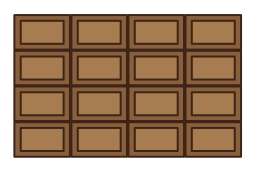
\includegraphics[width=.6\textwidth, keepaspectratio]{../../livro/media/cap2/secoes/pngs_licao_02/ativ3_fig01.png} 
\end{center}

\begin{enumerate} [\quad a)] %s
  \item     Que fração de uma torta é uma fatia? Explique.
  \item     Domingo papai comprou 4 fatias, quantos oitavos de uma torta havia para a sobremesa?
  \item     Na pergunta anterior, apresente outra fração que represente a quantidade de torta que papai comprou. Explique sua resposta.
  \item     Hoje papai comprou 10 fatias de torta. Como podemos representar essa quantidade de torta em termos de frações de     {\bf uma torta}    ? Lembre-se que oito fatias formam uma torta inteira.
\end{enumerate} %s

\subsection{Atividade}

Complete as afirmações com uma das frações: ``dois meios'', ``dois terços'', ``dois quintos'', ``três quartos'', ``oito sextos'' e ``nove meios'' para que sejam verdadeiras.

\begin{enumerate}[a)]
 \item A parte pintada de vermelho em \begin{tikzpicture}[scale=0.8]
                           \draw[fill=attention] (0,0) rectangle (20,10);
                           \draw[fill=common, fill opacity=.3] (20,0) rectangle (30,10);
                          \end{tikzpicture} 
                          é \begin{tikzpicture}
                             \draw (0,0) -- (20,0);
                            \end{tikzpicture}
                            de \begin{tikzpicture}[scale=0.8]
                                 \draw[fill=common, fill opacity=.3] (0,0) rectangle (30,10);
                               \end{tikzpicture}.

 \item A parte pintada de vermelho em \begin{tikzpicture}
                           \draw[fill=attention] (0,0) rectangle (8,8);
                           \draw (0,0) -- (8,8);
                          \end{tikzpicture} 
                          é \begin{tikzpicture}
                             \draw (0,0) -- (20,0);
                            \end{tikzpicture}
                            de \begin{tikzpicture}
                            \draw[fill=common, fill opacity=.3] (0,0) rectangle (8,8);                           
                           \end{tikzpicture}. 


 \item A parte pintada de vermelho em \begin{tikzpicture}
                           \draw[fill=common, fill opacity=.3] (0,0) circle (4);
                           \fill[attention] (0,0) -- (72:4) arc (72:-72:4) --cycle;
                           \foreach \x in {0,72,...,288}{
                           \draw (0,0) -- (\x:4);}                           
                          \end{tikzpicture} 
                          é \begin{tikzpicture}
                             \draw (0,0) -- (20,0);
                            \end{tikzpicture}
                            de \begin{tikzpicture}
                            \draw[fill=common, fill opacity=.3] (0,0) circle (4);                           
                           \end{tikzpicture}.            

 \item A parte pintada de vermelho em \begin{tikzpicture}
                                       \fill[attention]  \foreach \x/\y in {36/72,108/144,180/212, 252/284, 324/360}{ (0,0) -- (\x-18:4) -- (\y-18:2)--(\x-18 +72:4) -- (0, 0)};
                                       \draw  \foreach \x/\y in {36/72,108/144,180/212, 252/284, 324/360}{ (\x-18:4) -- (\y-18:2)--(\x-18 +72:4)};
                                      \end{tikzpicture} \begin{tikzpicture}
                                       \fill[attention]  \foreach \x/\y in {36/72,108/144,180/212, 252/284, 324/360}{ (0,0) -- (\x-18:4) -- (\y-18:2)--(\x-18 +72:4) -- (0, 0)};
                                       \draw  \foreach \x/\y in {36/72,108/144,180/212, 252/284, 324/360}{ (\x-18:4) -- (\y-18:2)--(\x-18 +72:4)};
                                      \end{tikzpicture} \begin{tikzpicture}
                                       \fill[attention]  \foreach \x/\y in {36/72,108/144,180/212, 252/284, 324/360}{ (0,0) -- (\x-18:4) -- (\y-18:2)--(\x-18 +72:4) -- (0, 0)};
                                       \draw  \foreach \x/\y in {36/72,108/144,180/212, 252/284, 324/360}{ (\x-18:4) -- (\y-18:2)--(\x-18 +72:4)};
                                      \end{tikzpicture} \begin{tikzpicture}
                                       \fill[attention]  \foreach \x/\y in {36/72,108/144,180/212, 252/284, 324/360}{ (0,0) -- (\x-18:4) -- (\y-18:2)--(\x-18 +72:4) -- (0, 0)};
                                       \draw  \foreach \x/\y in {36/72,108/144,180/212, 252/284, 324/360}{ (\x-18:4) -- (\y-18:2)--(\x-18 +72:4)};
                                      \end{tikzpicture} \begin{tikzpicture}
                                       \fill[attention]  \foreach \x/\y in {36/72,108/144,180/212, 252/284, 324/360}{ (0,0) -- (\x-18:4) -- (\y-18:2)--(\x-18 +72:4) -- (0, 0)};
                                       \fill[white]  (90:4) -- (-90:2) -- (-56:4) -- (-18:2)-- (18:4) --(56:2) --cycle;
                                       \fill[common, opacity=.3]  (90:4) -- (-90:2) -- (-56:4) -- (-18:2)-- (18:4) --(56:2) --cycle;
                                       \draw  \foreach \x/\y in {36/72,108/144,180/212, 252/284, 324/360}{ (\x-18:4) -- (\y-18:2)--(\x-18 +72:4)};
                                      \end{tikzpicture} é \begin{tikzpicture} \draw (0,0) -- (20,0); \end{tikzpicture} de \begin{tikzpicture}
                                       \fill[common, opacity=.3]  \foreach \x/\y in {36/72,108/144,180/212, 252/284, 324/360}{ (0,0) -- (\x-18:4) -- (\y-18:2)--(\x-18 +72:4) -- (0, 0)};
                                       \draw  \foreach \x/\y in {36/72,108/144,180/212, 252/284, 324/360}{ (\x-18:4) -- (\y-18:2)--(\x-18 +72:4)};
                                      \end{tikzpicture}.

\item A parte pintada de vermelho em \begin{tikzpicture} \draw[fill=attention] (90:4)--(-90:4)--(-30:4)--(30:4)--cycle; \foreach \x in {30,90,...,330}{\draw (0,0) -- (\x:4);} \draw[fill=common, fill opacity=.3] (90:4) -- (150:4) -- (210:4) -- (270:4) -- cycle;\end{tikzpicture} \begin{tikzpicture} \fill[attention] (30:4)--(90:4)--(150:4)--(210:4)--(270:4)-- (330:4) -- (0,0) --cycle; \foreach \x in {30,90,...,330}{\draw (0,0) -- (\x:4); \draw (\x:4) -- (\x+60:4);} \fill[common, fill opacity=.3] (0,0) -- (30:4) -- (-30:4) -- cycle;\end{tikzpicture} é \begin{tikzpicture} \draw (0,0) -- (20,0); \end{tikzpicture} de \begin{tikzpicture} \draw[fill=common, fill opacity=.3] (30:4) --(90:4)--(150:4)--(210:4)--(270:4)-- (330:4) -- cycle;\end{tikzpicture}.                  
\end{enumerate}

\section{ORGANIZANDO AS IDEIAS }

Se uma torta está dividida em três partes iguais, a torta fica separada em três terços. Assim, como visto na historinha do início da lição, tanto faz escrever: ``$\frac{1}{3}$ da torta'' ou ``um terço da torta'' para se referir à fatia destacada na figura.

\begin{center}
\begin{tikzpicture}
 \draw[fill=common, fill opacity=.3] (0,0) circle (10);
 \draw[fill=attention] (0,0) -- (-90:10) arc (-90:30:10) -- (0,0) -- cycle;
 \draw (0,0) -- (-90:10);
 \draw (0,0) -- (30:10);
 \draw (0,0) -- (150:10);
 \node at (0,-14) {$\frac{1}{3}$ da torta};
\end{tikzpicture}
\end{center}


Duas fatias são ``dois terços da torta'', o que pode ser expresso simplesmente por ``$\frac{2}{3}$ da torta''. Deste modo, é claro que ``três terços da torta'' é uma torta inteira.

\begin{center}
\begin{tikzpicture}
 \draw[fill=common, fill opacity=.3] (0,0) circle (10);
 \draw[fill=attention] (0,0) -- (-210:10) arc (-210:30:10) -- (0,0) -- cycle;
 \draw (0,0) circle (10);
 \draw (0,0) -- (-90:10);
 \draw (0,0) -- (30:10);
 \draw (0,0) -- (150:10);
 \node at (0,-14) {$\frac{2}{3}$ da torta};
\end{tikzpicture}\quad \quad \quad \begin{tikzpicture}
 \draw[fill=attention] (0,0) circle (10);
 \draw (0,0) -- (-90:10);
 \draw (0,0) -- (30:10);
 \draw (0,0) -- (150:10);
 \node at (0,-14) {$\frac{3}{3}$ da torta};
\end{tikzpicture}
\end{center}
  
  
Também pode-se considerar quatro terços, cinco terços ou seis terços da torta, basta juntar novos terços à torta inteira.

\begin{center}
\begin{tikzpicture}
\begin{scope}[shift={(-24,0)}]
 \draw[fill=attention] (0,0) circle (10);
 \draw (0,0) -- (-90:10);
 \draw (0,0) -- (30:10);
 \draw (0,0) -- (150:10);
 \end{scope}
 \draw[fill=attention] (0,0) -- (150:10) arc (150:30:10) -- (0,0) -- cycle;
 \node at (-12,-14) {$\frac{4}{3}$ da torta = 1 torta e $\frac{1}{3}$ da torta};
\end{tikzpicture}
\vspace{0.4cm}

\begin{tikzpicture}
\begin{scope}[shift={(-24,0)}]
 \draw[fill=attention] (0,0) circle (10);
 \draw (0,0) -- (-90:10);
 \draw (0,0) -- (30:10);
 \draw (0,0) -- (150:10);
 \end{scope}
 \draw[fill=attention] (0,0) -- (150:10) arc (150:-90:10) -- (0,0) -- cycle;
 \draw (0,0) -- (30:10);
 \node at (-12,-14) {$\frac{5}{3}$ da torta = 1 torta e $\frac{2}{3}$ da torta};
\end{tikzpicture}
\vspace{0.4cm}

\begin{tikzpicture}
\begin{scope}[shift={(-24,0)}]
 \draw[fill=attention] (0,0) circle (10);
 \draw (0,0) -- (-90:10);
 \draw (0,0) -- (30:10);
 \draw (0,0) -- (150:10);
 \end{scope}
 \draw[fill=attention] (0,0) circle (10);
 \draw (0,0) -- (-90:10);
 \draw (0,0) -- (30:10);
 \draw (0,0) -- (150:10);
 \node at (-12,-14) {$\frac{6}{3}$ da torta = 2 tortas};
\end{tikzpicture}
\end{center}

Se uma torta é repartida em três partes iguais, cada fatia é um terço da torta - ou, simplesmente, $\frac{1}{3}$ da torta. Juntando essas fatias, é possível se ter dois terços ($\frac{2}{3}$) e três terços ($\frac{3}{3}$) da torta. Com mais do que uma torta repartida em três partes iguais, obtem-se quatro terços ($\frac{4}{3}$), cinco terços ($\frac{5}{3}$), seis terços ($\frac{6}{3}$), etc, da torta. Na representação simbólica, as frações que registram essas quantidades têm o número 3 ``abaixo'' do traço de fração, e, por isso, são denominadas terços. O número que informa a parte da unidade que ``dá nome'' à fração é chamado de {\it denominador} da fração. Assim, nas frações $\frac{1}{3}$, $\frac{2}{3}$, $\frac{3}{3}$,  $\frac{4}{3}$ e $\frac{5}{3}$, o 3 é o denominador, identificando ``terços''. 

Já o número que aparece ``acima'' do traço de fração informa quantos terços estão sendo considerados. Esse número é chamado de {\it numerador} da fração. Por exemplo, na fração $\frac{1}{3}$ o numerador é 1 e na fração $\frac{4}{3}$ o numerador é 4.

Essa mesma forma de nomear vale para outras frações, mesmo que o denominador seja diferente de 3:\mbox{} \newline 
Em $\frac{2}{5}$, por exemplo, o numerador é 2 e o denominador é 5. Fala-se {\it dois quintos}.\mbox{} \newline 
Em $\frac{10}{8}$, por exemplo, o numerador é 10 e o denominador é 8. Fala-se {\it dez oitavos}. \mbox{} \newline 
Como você pôde observar, a nomeação de uma fração depende fortemente do denominador da fração. Para ler a fração basta lermos o {\bf número} do numerador seguido do {\bf nome que identifica a fração do tipo} $\frac{1}{b}$, nessa ordem. Veja:

$$\frac{1}{3}\rightarrow \text{ um terço;} \quad \frac{2}{3}\rightarrow \text{ dois terços;} \quad \frac{5}{3}\rightarrow \text{ cinco terços;}$$
$$\frac{1}{8}\rightarrow \text{ um oitavo;} \quad \frac{3}{8}\rightarrow \text{ três oitavos;} \quad \frac{7}{8}\rightarrow \text{ sete oitavos.}$$
Anote agora os nomes de algumas outras frações:
$$\frac{1}{2}\rightarrow \text{  um meio;} \quad \frac{1}{3}\rightarrow\text{  um terço;} \quad \frac{1}{4}\rightarrow\text{  um quarto;}$$
$$\frac{1}{5}\rightarrow\text{  um quinto;}\quad \frac{1}{6}\rightarrow\text{  um sexto;} \quad \frac{1}{7}\rightarrow\text{  um sétimo;}$$
$$\frac{1}{8}\rightarrow\text{  um oitavo;}\quad \frac{1}{9}\rightarrow\text{  um nono;}\quad \frac{1}{10}\rightarrow\text{  um décimo.}$$

Para a fração $\frac{1}{11}$, fala-se um onze avos. Da mesma forma, são nomeadas frações cujo denominador é maior do que 11. Por exemplo:
$$\frac{1}{12}\rightarrow \text{  um doze avos;}\quad \frac{1}{13}\rightarrow \text{ um treze avos;} \quad \frac{5}{13}\rightarrow \text{ cinco treze avos.}$$

Curioso para saber sobre o significado da palavra {\bf avos}? Pergunte ao seu professor. O importante é lembrar que, para denominadores maiores 11, acrescenta-se a expressão ``avos'' ao final da leitura da fração.

Contudo, para frações cujo denominador é uma potência de 10, usa-se outra formar de ler:
$$\frac{1}{100}\rightarrow \text{ um centésimo;}\quad \frac{13}{100} \rightarrow \text{treze centésimos;} \quad
\frac{33}{1000}\rightarrow \text{ trinta e três milésimos.}$$

{\bf Pronto! Agora você já é capaz de ler diversos tipos de frações.}

\begin{center}
 
\includegraphics[width=.9\textwidth, keepaspectratio]{../../livro/media/cap2/secoes/pngs_licao_02/orgideias_fig01.png} 
\end{center}


\section{MÃO NA MASSA }

\subsection{Atividade}

Uma pizza gigante foi dividida em doze fatias iguais. 
Pedro comeu quatro fatias, Isabella cinco fatias, Bernardo duas fatias e Manuela apenas uma fatia.

\begin{center}
  \begin{tabular}{|m{0.27\textwidth}|m{0.13\textwidth}|m{0.13\textwidth}|m{0.13\textwidth}|m{0.13\textwidth}|}
\hline  
& \centering Pedro & \centering  Isabella & \centering  Bernardo &  \quad Manuela  \\
    \hline  \hline
   Pinte a fração de pizza consumida  por cada pessoa      & \parbox[c][2cm]{0.13\textwidth}{\centering 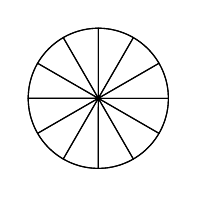
\begin{tikzpicture}[x=1.0cm,y=1.0cm, scale=0.5]
\draw (1.76,2.04) circle (1.78cm);
\draw [shift={(1.76,2.04)}]  (0,0) --  plot[domain=0.:0.5235987755982987,variable=\t]({1.*1.78*cos(\t r)+0.*1.78*sin(\t r)},{0.*1.78*cos(\t r)+1.*1.78*sin(\t r)}) -- cycle ;
\draw [shift={(1.76,2.04)}]  (0,0) --  plot[domain=0.5235987755982987:1.0471975511965974,variable=\t]({1.*1.78*cos(\t r)+0.*1.78*sin(\t r)},{0.*1.78*cos(\t r)+1.*1.78*sin(\t r)}) -- cycle ;
\draw [shift={(1.76,2.04)}]  (0,0) --  plot[domain=1.0471975511965974:1.5707963267948963,variable=\t]({1.*1.78*cos(\t r)+0.*1.78*sin(\t r)},{0.*1.78*cos(\t r)+1.*1.78*sin(\t r)}) -- cycle ;
\draw [shift={(1.76,2.04)}]  (0,0) --  plot[domain=1.5707963267948963:2.0943951023931953,variable=\t]({1.*1.78*cos(\t r)+0.*1.78*sin(\t r)},{0.*1.78*cos(\t r)+1.*1.78*sin(\t r)}) -- cycle ;
\draw [shift={(1.76,2.04)}]  (0,0) --  plot[domain=2.0943951023931953:2.617993877991494,variable=\t]({1.*1.78*cos(\t r)+0.*1.78*sin(\t r)},{0.*1.78*cos(\t r)+1.*1.78*sin(\t r)}) -- cycle ;
\draw [shift={(1.76,2.04)}]  (0,0) --  plot[domain=2.617993877991494:3.1415926535897927,variable=\t]({1.*1.78*cos(\t r)+0.*1.78*sin(\t r)},{0.*1.78*cos(\t r)+1.*1.78*sin(\t r)}) -- cycle ;
\draw [shift={(1.76,2.04)}]  (0,0) --  plot[domain=3.1415926535897927:3.6651914291880914,variable=\t]({1.*1.78*cos(\t r)+0.*1.78*sin(\t r)},{0.*1.78*cos(\t r)+1.*1.78*sin(\t r)}) -- cycle ;
\draw [shift={(1.76,2.04)}]  (0,0) --  plot[domain=3.6651914291880914:4.18879020478639,variable=\t]({1.*1.78*cos(\t r)+0.*1.78*sin(\t r)},{0.*1.78*cos(\t r)+1.*1.78*sin(\t r)}) -- cycle ;
\draw [shift={(1.76,2.04)}]  (0,0) --  plot[domain=4.18879020478639:4.712388980384689,variable=\t]({1.*1.78*cos(\t r)+0.*1.78*sin(\t r)},{0.*1.78*cos(\t r)+1.*1.78*sin(\t r)}) -- cycle ;
\draw [shift={(1.76,2.04)}]  (0,0) --  plot[domain=4.712388980384689:5.235987755982988,variable=\t]({1.*1.78*cos(\t r)+0.*1.78*sin(\t r)},{0.*1.78*cos(\t r)+1.*1.78*sin(\t r)}) -- cycle ;
\draw [shift={(1.76,2.04)}]  (0,0) --  plot[domain=5.235987755982988:5.759586531581286,variable=\t]({1.*1.78*cos(\t r)+0.*1.78*sin(\t r)},{0.*1.78*cos(\t r)+1.*1.78*sin(\t r)}) -- cycle ;
\draw [shift={(1.76,2.04)}]  (0,0) --  plot[domain=-0.5235987755983:0.,variable=\t]({1.*1.78*cos(\t r)+0.*1.78*sin(\t r)},{0.*1.78*cos(\t r)+1.*1.78*sin(\t r)}) -- cycle ;
\end{tikzpicture}}
  & \parbox[c][2cm]{0.13\textwidth}{\centering 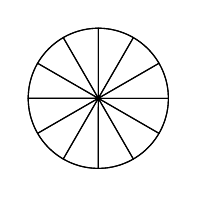
\begin{tikzpicture}[x=1.0cm,y=1.0cm, scale=0.5]
\draw (1.76,2.04) circle (1.78cm);
\draw [shift={(1.76,2.04)}]  (0,0) --  plot[domain=0.:0.5235987755982987,variable=\t]({1.*1.78*cos(\t r)+0.*1.78*sin(\t r)},{0.*1.78*cos(\t r)+1.*1.78*sin(\t r)}) -- cycle ;
\draw [shift={(1.76,2.04)}]  (0,0) --  plot[domain=0.5235987755982987:1.0471975511965974,variable=\t]({1.*1.78*cos(\t r)+0.*1.78*sin(\t r)},{0.*1.78*cos(\t r)+1.*1.78*sin(\t r)}) -- cycle ;
\draw [shift={(1.76,2.04)}]  (0,0) --  plot[domain=1.0471975511965974:1.5707963267948963,variable=\t]({1.*1.78*cos(\t r)+0.*1.78*sin(\t r)},{0.*1.78*cos(\t r)+1.*1.78*sin(\t r)}) -- cycle ;
\draw [shift={(1.76,2.04)}]  (0,0) --  plot[domain=1.5707963267948963:2.0943951023931953,variable=\t]({1.*1.78*cos(\t r)+0.*1.78*sin(\t r)},{0.*1.78*cos(\t r)+1.*1.78*sin(\t r)}) -- cycle ;
\draw [shift={(1.76,2.04)}]  (0,0) --  plot[domain=2.0943951023931953:2.617993877991494,variable=\t]({1.*1.78*cos(\t r)+0.*1.78*sin(\t r)},{0.*1.78*cos(\t r)+1.*1.78*sin(\t r)}) -- cycle ;
\draw [shift={(1.76,2.04)}]  (0,0) --  plot[domain=2.617993877991494:3.1415926535897927,variable=\t]({1.*1.78*cos(\t r)+0.*1.78*sin(\t r)},{0.*1.78*cos(\t r)+1.*1.78*sin(\t r)}) -- cycle ;
\draw [shift={(1.76,2.04)}]  (0,0) --  plot[domain=3.1415926535897927:3.6651914291880914,variable=\t]({1.*1.78*cos(\t r)+0.*1.78*sin(\t r)},{0.*1.78*cos(\t r)+1.*1.78*sin(\t r)}) -- cycle ;
\draw [shift={(1.76,2.04)}]  (0,0) --  plot[domain=3.6651914291880914:4.18879020478639,variable=\t]({1.*1.78*cos(\t r)+0.*1.78*sin(\t r)},{0.*1.78*cos(\t r)+1.*1.78*sin(\t r)}) -- cycle ;
\draw [shift={(1.76,2.04)}]  (0,0) --  plot[domain=4.18879020478639:4.712388980384689,variable=\t]({1.*1.78*cos(\t r)+0.*1.78*sin(\t r)},{0.*1.78*cos(\t r)+1.*1.78*sin(\t r)}) -- cycle ;
\draw [shift={(1.76,2.04)}]  (0,0) --  plot[domain=4.712388980384689:5.235987755982988,variable=\t]({1.*1.78*cos(\t r)+0.*1.78*sin(\t r)},{0.*1.78*cos(\t r)+1.*1.78*sin(\t r)}) -- cycle ;
\draw [shift={(1.76,2.04)}]  (0,0) --  plot[domain=5.235987755982988:5.759586531581286,variable=\t]({1.*1.78*cos(\t r)+0.*1.78*sin(\t r)},{0.*1.78*cos(\t r)+1.*1.78*sin(\t r)}) -- cycle ;
\draw [shift={(1.76,2.04)}]  (0,0) --  plot[domain=-0.5235987755983:0.,variable=\t]({1.*1.78*cos(\t r)+0.*1.78*sin(\t r)},{0.*1.78*cos(\t r)+1.*1.78*sin(\t r)}) -- cycle ;
\end{tikzpicture}}
   & \parbox[c][2cm]{0.13\textwidth}{\centering 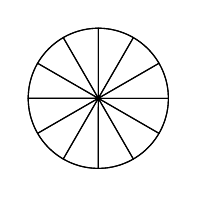
\begin{tikzpicture}[x=1.0cm,y=1.0cm, scale=0.5]
\draw (1.76,2.04) circle (1.78cm);
\draw [shift={(1.76,2.04)}]  (0,0) --  plot[domain=0.:0.5235987755982987,variable=\t]({1.*1.78*cos(\t r)+0.*1.78*sin(\t r)},{0.*1.78*cos(\t r)+1.*1.78*sin(\t r)}) -- cycle ;
\draw [shift={(1.76,2.04)}]  (0,0) --  plot[domain=0.5235987755982987:1.0471975511965974,variable=\t]({1.*1.78*cos(\t r)+0.*1.78*sin(\t r)},{0.*1.78*cos(\t r)+1.*1.78*sin(\t r)}) -- cycle ;
\draw [shift={(1.76,2.04)}]  (0,0) --  plot[domain=1.0471975511965974:1.5707963267948963,variable=\t]({1.*1.78*cos(\t r)+0.*1.78*sin(\t r)},{0.*1.78*cos(\t r)+1.*1.78*sin(\t r)}) -- cycle ;
\draw [shift={(1.76,2.04)}]  (0,0) --  plot[domain=1.5707963267948963:2.0943951023931953,variable=\t]({1.*1.78*cos(\t r)+0.*1.78*sin(\t r)},{0.*1.78*cos(\t r)+1.*1.78*sin(\t r)}) -- cycle ;
\draw [shift={(1.76,2.04)}]  (0,0) --  plot[domain=2.0943951023931953:2.617993877991494,variable=\t]({1.*1.78*cos(\t r)+0.*1.78*sin(\t r)},{0.*1.78*cos(\t r)+1.*1.78*sin(\t r)}) -- cycle ;
\draw [shift={(1.76,2.04)}]  (0,0) --  plot[domain=2.617993877991494:3.1415926535897927,variable=\t]({1.*1.78*cos(\t r)+0.*1.78*sin(\t r)},{0.*1.78*cos(\t r)+1.*1.78*sin(\t r)}) -- cycle ;
\draw [shift={(1.76,2.04)}]  (0,0) --  plot[domain=3.1415926535897927:3.6651914291880914,variable=\t]({1.*1.78*cos(\t r)+0.*1.78*sin(\t r)},{0.*1.78*cos(\t r)+1.*1.78*sin(\t r)}) -- cycle ;
\draw [shift={(1.76,2.04)}]  (0,0) --  plot[domain=3.6651914291880914:4.18879020478639,variable=\t]({1.*1.78*cos(\t r)+0.*1.78*sin(\t r)},{0.*1.78*cos(\t r)+1.*1.78*sin(\t r)}) -- cycle ;
\draw [shift={(1.76,2.04)}]  (0,0) --  plot[domain=4.18879020478639:4.712388980384689,variable=\t]({1.*1.78*cos(\t r)+0.*1.78*sin(\t r)},{0.*1.78*cos(\t r)+1.*1.78*sin(\t r)}) -- cycle ;
\draw [shift={(1.76,2.04)}]  (0,0) --  plot[domain=4.712388980384689:5.235987755982988,variable=\t]({1.*1.78*cos(\t r)+0.*1.78*sin(\t r)},{0.*1.78*cos(\t r)+1.*1.78*sin(\t r)}) -- cycle ;
\draw [shift={(1.76,2.04)}]  (0,0) --  plot[domain=5.235987755982988:5.759586531581286,variable=\t]({1.*1.78*cos(\t r)+0.*1.78*sin(\t r)},{0.*1.78*cos(\t r)+1.*1.78*sin(\t r)}) -- cycle ;
\draw [shift={(1.76,2.04)}]  (0,0) --  plot[domain=-0.5235987755983:0.,variable=\t]({1.*1.78*cos(\t r)+0.*1.78*sin(\t r)},{0.*1.78*cos(\t r)+1.*1.78*sin(\t r)}) -- cycle ;
\end{tikzpicture}}
  & \parbox[c][2cm]{0.13\textwidth}{\centering 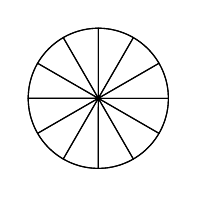
\begin{tikzpicture}[x=1.0cm,y=1.0cm, scale=0.5]
\draw (1.76,2.04) circle (1.78cm);
\draw [shift={(1.76,2.04)}]  (0,0) --  plot[domain=0.:0.5235987755982987,variable=\t]({1.*1.78*cos(\t r)+0.*1.78*sin(\t r)},{0.*1.78*cos(\t r)+1.*1.78*sin(\t r)}) -- cycle ;
\draw [shift={(1.76,2.04)}]  (0,0) --  plot[domain=0.5235987755982987:1.0471975511965974,variable=\t]({1.*1.78*cos(\t r)+0.*1.78*sin(\t r)},{0.*1.78*cos(\t r)+1.*1.78*sin(\t r)}) -- cycle ;
\draw [shift={(1.76,2.04)}]  (0,0) --  plot[domain=1.0471975511965974:1.5707963267948963,variable=\t]({1.*1.78*cos(\t r)+0.*1.78*sin(\t r)},{0.*1.78*cos(\t r)+1.*1.78*sin(\t r)}) -- cycle ;
\draw [shift={(1.76,2.04)}]  (0,0) --  plot[domain=1.5707963267948963:2.0943951023931953,variable=\t]({1.*1.78*cos(\t r)+0.*1.78*sin(\t r)},{0.*1.78*cos(\t r)+1.*1.78*sin(\t r)}) -- cycle ;
\draw [shift={(1.76,2.04)}]  (0,0) --  plot[domain=2.0943951023931953:2.617993877991494,variable=\t]({1.*1.78*cos(\t r)+0.*1.78*sin(\t r)},{0.*1.78*cos(\t r)+1.*1.78*sin(\t r)}) -- cycle ;
\draw [shift={(1.76,2.04)}]  (0,0) --  plot[domain=2.617993877991494:3.1415926535897927,variable=\t]({1.*1.78*cos(\t r)+0.*1.78*sin(\t r)},{0.*1.78*cos(\t r)+1.*1.78*sin(\t r)}) -- cycle ;
\draw [shift={(1.76,2.04)}]  (0,0) --  plot[domain=3.1415926535897927:3.6651914291880914,variable=\t]({1.*1.78*cos(\t r)+0.*1.78*sin(\t r)},{0.*1.78*cos(\t r)+1.*1.78*sin(\t r)}) -- cycle ;
\draw [shift={(1.76,2.04)}]  (0,0) --  plot[domain=3.6651914291880914:4.18879020478639,variable=\t]({1.*1.78*cos(\t r)+0.*1.78*sin(\t r)},{0.*1.78*cos(\t r)+1.*1.78*sin(\t r)}) -- cycle ;
\draw [shift={(1.76,2.04)}]  (0,0) --  plot[domain=4.18879020478639:4.712388980384689,variable=\t]({1.*1.78*cos(\t r)+0.*1.78*sin(\t r)},{0.*1.78*cos(\t r)+1.*1.78*sin(\t r)}) -- cycle ;
\draw [shift={(1.76,2.04)}]  (0,0) --  plot[domain=4.712388980384689:5.235987755982988,variable=\t]({1.*1.78*cos(\t r)+0.*1.78*sin(\t r)},{0.*1.78*cos(\t r)+1.*1.78*sin(\t r)}) -- cycle ;
\draw [shift={(1.76,2.04)}]  (0,0) --  plot[domain=5.235987755982988:5.759586531581286,variable=\t]({1.*1.78*cos(\t r)+0.*1.78*sin(\t r)},{0.*1.78*cos(\t r)+1.*1.78*sin(\t r)}) -- cycle ;
\draw [shift={(1.76,2.04)}]  (0,0) --  plot[domain=-0.5235987755983:0.,variable=\t]({1.*1.78*cos(\t r)+0.*1.78*sin(\t r)},{0.*1.78*cos(\t r)+1.*1.78*sin(\t r)}) -- cycle ;
\end{tikzpicture}}
  \\
    \hline
     Escreva, por extenso, a fração de pizza consumida por cada pessoa&                                        &                                        &                                         &                                        \\
    \hline
     Escreva, usando notação simbólica matemática, a fração de pizza consumida por cada pessoa &                                        &                                        &                                         &                                        \\
    \hline
  \end{tabular}
\end{center}

\begin{enumerate} [\quad a)] %d
  \item     Na sua opinião, qual representação de fração     ``gasta menos lápis''     para se escrita? Usando notação simbólica matemática, escrevendo por extenso ou pintando?
  \item     Na sua opinião, qual a representação que mais rapidamente ajuda a decidir quem comeu mais e quem comeu menos pizza?
\end{enumerate} %d

\subsection{Atividade}

Para cada figura a seguir, indique a fração da figura que está pintada de vermelho. Esta fração é maior, menor ou exatamente igual a $\frac{1}{2}$ da figura?

\begin{center}
\begin{tabular}{m{0.3\textwidth}m{0.3\textwidth}m{0.3\textwidth}}

a)
\parbox[t][1.5cm][c]{5cm}{
\begin{tikzpicture}
\draw[fill=common, fill opacity=.3] (0,0) circle (10);
 \foreach \x in {0,72,...,288}{
 \draw[fill=attention] (0,0) -- (\x:10) arc (\x:\x+36:10) --cycle;
 \draw (\x:10) -- (\x:-10);}
\end{tikzpicture} }
&
b)
\parbox[t][1.5cm][c]{5cm}{
\begin{tikzpicture}
\draw[fill=common, fill opacity=.3] (0,0) rectangle (14,20);
\draw[fill=attention] (0,4) rectangle (7,20);
\foreach \y in {4,8,12,16}{
\draw (0,\y)--(14,\y);}
\draw (7,0) -- (7,20);
\end{tikzpicture} }

&

c)
\parbox[t][1.5cm][c]{5cm}{
\begin{tikzpicture}
\draw[fill=common, fill opacity=.3] (0,0) rectangle (30,20);
\fill[attention] (0,0) rectangle (18,20);
 \foreach \x in {3,6,...,27}{
 \draw (\x,0)--(\x,20);}
\end{tikzpicture} }

\end{tabular}
\end{center}

\subsection{Atividade}

Um grupo de amigos está dividindo duas pizzas circulares do mesmo tamanho. A primeira pizza foi cortada em 4 fatias de mesmo tamanho. A segunda pizza foi dividida em 8 fatias iguais.

\begin{enumerate} [\quad a)] %s
  \item     Uma fatia da primeira pizza é que fração dessa pizza? Responda usando notação simbólica matemática.
  \item     Uma fatia da segunda pizza é que fração dessa pizza? Responda usando notação simbólica matemática.
  \item     Qual fatia tem mais quantidade de pizza: uma fatia da primeira pizza ou uma fatia da segunda? Explique usando um desenho.
\end{enumerate} %s

\subsection{Atividade}

Preencha cada lacuna a seguir com uma fração adequada (use notação simbólica matemática). Perceba que uma mesma parte pintada pode ser descrita por frações diferentes com unidades diferentes.

%definição da região limitada pelos 2 hexágonos encaixados.
\def \tripinha{ (30:4) -- (90:4) -- (150:4)--(210:4)--(270:4)--(330:4) [shift={({4*sqrt(3)},0)}] --(270:4) -- (330:4) -- (30:4) -- (90:4)--(150:4)--cycle;}
%definição da região limitada pelos 3 hexágonos encaixados.
\def \tripa{ (30:4) -- (90:4) -- (150:4)--(210:4)--(270:4)--(330:4) [shift={({4*sqrt(3)},0)}] --(270:4) -- (330:4) [shift={({4*sqrt(3)},0)}]--  (270:4) -- (330:4) -- (30:4) -- (90:4)--(150:4) [shift={({-4*sqrt(3)},0)}] -- (90:4) -- (150:4)--cycle;}

\begin{enumerate} [\quad a)] %s
%a
\item     A parte pintada em vermelho em  
\begin{tikzpicture}[scale=1.3]
 \draw \tripa;
\begin{scope}
 \clip \tripa;
\draw[fill=attention] (-4,-4) rectangle (0,4);
\draw[fill=common, fill opacity=.3] (0,-4) rectangle (20,4);
\end{scope}
\end{tikzpicture} 
é 
\begin{tikzpicture} \draw (0,0)--(20,0);\end{tikzpicture}   
de  
\begin{tikzpicture}[scale=1.3]
\draw[fill=common, fill opacity=.3] (30:4) -- (90:4) -- (150:4) -- (210:4) -- (270:4) -- (330:4)--cycle;
\end{tikzpicture}.
 %b 
\item     A parte pintada em vermelho em 
\begin{tikzpicture}[scale=1.3]
 \draw \tripa;
\begin{scope}
 \clip \tripa;
\draw[fill=attention] (-4,-4) rectangle (0,4);
\draw[fill=common, fill opacity=.3] (0,-4) rectangle (20,4);
\end{scope}
\end{tikzpicture} 
é 
\begin{tikzpicture} \draw (0,0)--(20,0);\end{tikzpicture}
de
\begin{tikzpicture}[scale=1.3]
 \draw[fill=common, fill opacity=.3] (30:4) -- (90:4) -- (150:4)--(210:4)--(270:4)--(330:4) [shift={({4*sqrt(3)},0)}] --(270:4) -- (330:4) --(30:4) -- (90:4) -- (150:4)--cycle;
\end{tikzpicture}.

%c
\item     A parte pintada em vermelho em \begin{tikzpicture}[scale=1.3]
 \draw \tripa;
\begin{scope}
 \clip \tripa;
\draw[fill=attention] (-4,-4) rectangle (0,4);
\draw[fill=common, fill opacity=.3] (0,-4) rectangle (20,4);
\end{scope}
\end{tikzpicture} 
     é \begin{tikzpicture} \draw (0,0)--(20,0);\end{tikzpicture}    de  
\begin{tikzpicture}[scale=1.3]
\draw[fill=common, fill opacity=.3] \tripa;
\end{tikzpicture}.

%d                                            
 \item     A parte pintada em vermelho em  \begin{tikzpicture}[scale=1.3]
 \draw \tripa;
\begin{scope}
 \clip \tripa;
\draw[fill=attention] (-4,-4) rectangle ({4*sqrt(3)},4);
\draw[fill=common, fill opacity=.3] ({4*sqrt(3)},-4) rectangle ({10*sqrt(3)},4);
\end{scope}
\end{tikzpicture}  é \begin{tikzpicture} \draw (0,0)--(20,0);\end{tikzpicture}    de
\begin{tikzpicture}[scale=1.3]
\draw[fill=common, fill opacity=.3] (30:4) -- (90:4) -- (150:4) -- (210:4) -- (270:4) -- (330:4)--cycle;
\end{tikzpicture}.
%e
\item     A parte pintada em vermelho em   \begin{tikzpicture}[scale=1.3]
 \draw \tripa;
\begin{scope}
 \clip \tripa;
\draw[fill=attention] (-4,-4) rectangle ({4*sqrt(3)},4);
\draw[fill=common, fill opacity=.3] ({4*sqrt(3)},-4) rectangle ({10*sqrt(3)},4);
\end{scope}
\end{tikzpicture}    é \begin{tikzpicture} \draw (0,0)--(20,0);\end{tikzpicture}    de 
\begin{tikzpicture}[scale=1.3]
 \draw[fill=common, fill opacity=.3] (30:4) -- (90:4) -- (150:4)--(210:4)--(270:4)--(330:4) [shift={({4*sqrt(3)},0)}] --(270:4) -- (330:4) --(30:4) -- (90:4) -- (150:4)--cycle;
\end{tikzpicture}.

%f
\item     A parte pintada em vermelho em  \begin{tikzpicture}[scale=1.3]
 \draw \tripa;
\begin{scope}
 \clip \tripa;
\draw[fill=attention] (-4,-4) rectangle ({4*sqrt(3)},4);
\draw[fill=common, fill opacity=.3] ({4*sqrt(3)},-4) rectangle ({10*sqrt(3)},4);
\end{scope}
\end{tikzpicture}   é \begin{tikzpicture} \draw (0,0)--(20,0);\end{tikzpicture}    de 
\begin{tikzpicture}[scale=1.3]
\draw[fill=common, fill opacity=.3] \tripa;
\end{tikzpicture}.

%g
\item     A parte pintada em vermelho em  
\begin{tikzpicture}[scale=1.3]
 \draw \tripa;
\begin{scope}
 \clip \tripa;
\draw[fill=attention] (-4,-4) rectangle ({8*sqrt(3)},4);
\draw[fill=common, fill opacity=.3] ({8*sqrt(3)},-4) rectangle ({10*sqrt(3)},4);
\end{scope}
\end{tikzpicture}  
é \begin{tikzpicture} \draw (0,0)--(20,0);\end{tikzpicture}    de 
\begin{tikzpicture}[scale=1.3]
\draw[fill=common, fill opacity=.3] (30:4) -- (90:4) -- (150:4) -- (210:4) -- (270:4) -- (330:4)--cycle;
\end{tikzpicture}.
%h
\item     A parte pintada em vermelho em  \begin{tikzpicture}[scale=1.3]
 \draw \tripa;
\begin{scope}
 \clip \tripa;
\draw[fill=attention] (-4,-4) rectangle ({8*sqrt(3)},4);
\draw[fill=common, fill opacity=.3] ({8*sqrt(3)},-4) rectangle ({10*sqrt(3)},4);
\end{scope}
\end{tikzpicture} é \begin{tikzpicture} \draw (0,0)--(20,0);\end{tikzpicture}    de
\begin{tikzpicture}[scale=1.3]
 \draw[fill=common, fill opacity=.3] (30:4) -- (90:4) -- (150:4)--(210:4)--(270:4)--(330:4) [shift={({4*sqrt(3)},0)}] --(270:4) -- (330:4) --(30:4) -- (90:4) -- (150:4)--cycle;
\end{tikzpicture}.

%i
\item     A parte pintada em vermelho em   
\begin{tikzpicture}[scale=1.3]
 \draw \tripa;
\begin{scope}
 \clip \tripa;
\draw[fill=attention] (-4,-4) rectangle ({8*sqrt(3)},4);
\draw[fill=common, fill opacity=.3] ({8*sqrt(3)},-4) rectangle ({10*sqrt(3)},4);
\end{scope}
\end{tikzpicture}
é \begin{tikzpicture} \draw (0,0)--(20,0);\end{tikzpicture}    de 
\begin{tikzpicture}[scale=1.3]
\draw[fill=common, fill opacity=.3] \tripa;
\end{tikzpicture}.
%j
\item     A parte pintada em vermelho em 
  \begin{tikzpicture}[scale=1.3]
 \draw \tripa;
\begin{scope}
 \clip \tripa;
\draw[fill=attention] (-4,-4) rectangle ({12*sqrt(3)},4);
\end{scope}
\end{tikzpicture}
é \begin{tikzpicture} \draw (0,0)--(20,0);\end{tikzpicture}    de 
\begin{tikzpicture}[scale=1.3]
\draw[fill=common, fill opacity=.3] (30:4) -- (90:4) -- (150:4) -- (210:4) -- (270:4) -- (330:4)--cycle;
\end{tikzpicture}.
%k
\item     A parte pintada em vermelho em
\begin{tikzpicture}[scale=1.3]
 \draw \tripa;
\begin{scope}
 \clip \tripa;
\draw[fill=attention] (-4,-4) rectangle ({12*sqrt(3)},4);
\end{scope}
\end{tikzpicture}
é \begin{tikzpicture} \draw (0,0)--(20,0);\end{tikzpicture}    de 
\begin{tikzpicture}[scale=1.3]
 \draw[fill=common, fill opacity=.3] (30:4) -- (90:4) -- (150:4)--(210:4)--(270:4)--(330:4) [shift={({4*sqrt(3)},0)}] --(270:4) -- (330:4) --(30:4) -- (90:4) -- (150:4)--cycle;
\end{tikzpicture}.

%l
\item     A parte pintada em vermelho em  
  \begin{tikzpicture}[scale=1.3]
 \draw \tripa;
\begin{scope}
 \clip \tripa;
\draw[fill=attention] (-4,-4) rectangle ({12*sqrt(3)},4);
\end{scope}
\end{tikzpicture}
é \begin{tikzpicture} \draw (0,0)--(20,0);\end{tikzpicture}    de 
\begin{tikzpicture}[scale=1.3]
\draw[fill=common, fill opacity=.3] \tripa;
\end{tikzpicture}.


\end{enumerate} %s

\subsection{Atividade}

Na tabela a seguir, pinte cada figura de modo que a parte pintada seja a fração da figura indicada na coluna à esquerda na mesma linha. Indique também, usando notação simbólica matemática, qual fração da figura ficou sem pintar.

\begin{center}
  \begin{longtable}{|m{0.25\textwidth}|m{0.2\textwidth}|m{0.25\textwidth}|}
    \hline
      Fração da figura que deve ser pintada  & \centering  Figura  &   Fração da figura que ficou sem pintar  \\
    \hline \hline 
    \endhead
     \centering $\dfrac{5}{6}$  & \centering \parbox[c][1.75cm][c]{1.6cm}{\begin{tikzpicture}
                                    \foreach \x in {0,60,...,300}{ \draw (0,0)--(\x:8);\draw (\x:8)--(\x+60:8);}
                                   \end{tikzpicture}}
&  \\
    \hline 
     \centering $\dfrac{3}{4}$  &  \centering \parbox[c][1.75cm][c]{1.6cm}{\begin{tikzpicture}
                                    \draw (0:8)--(180:8);
                                    \draw (90:8)--(270:8);
                                    \draw (0,0) circle (8);
                                   \end{tikzpicture}}
                                   &  \\
    \hline 
     \centering $\dfrac{2}{5}$  &   \centering \parbox[c][1.75cm][c]{2.4cm}{
                                    \begin{tikzpicture}
                                    \draw (0,0) rectangle (25,16);
                                    \foreach \x in {5,10,15,20}{\draw (\x,0)--(\x,16);}
                                   \end{tikzpicture} }
                                   &  \\
    \hline
     \centering $\dfrac{2}{3}$  &  \centering \parbox[c][1.75cm][c]{1.6cm}{\begin{tikzpicture}
                                    \foreach \x in {0,60,...,300}{ \draw (0,0)--(\x:8);\draw (\x:8)--(\x+60:8);}
                                   \end{tikzpicture}}
                                   &  \\
    \hline
     \centering $\dfrac{3}{8}$  &   \centering \parbox[c][1.75cm][c]{1.6cm}{\begin{tikzpicture}
                                    \draw (0:8)--(180:8);
                                    \draw (90:8)--(270:8);
                                    \draw (0,0) circle (8);
                                   \end{tikzpicture}}&  \\
    \hline
     \centering $\dfrac{9}{10}$  & \centering \parbox[c][1.75cm][c]{2.4cm}{
                                    \begin{tikzpicture}
                                    \draw (0,0) rectangle (25,16);
                                    \foreach \x in {5,10,15,20}{\draw (\x,0)--(\x,16);}
                                   \end{tikzpicture} }
                                   &  \\
    \hline
  \end{longtable}
\end{center}

\subsection{Atividade}

\begin{enumerate} [\quad a)] %s
  \item     Em cada um dos três copos idênticos a seguir, indique a fração da capacidade do copo que está com água.
\begin{center}
\begin{tikzpicture}[scale=0.3, x=1cm,y=1cm]

% Definição do eixo vertical das elipses
\def\EixoM{0.5}

% colorindo o primeiro cilindro
\fill[common] (2,0) ellipse (2 and \EixoM);
\fill[common] (0,0) rectangle (4,3);
\fill[common] (2,3) ellipse (2 and \EixoM);

% colorindo o segundo cilindro
\fill[common] (8,0) ellipse (2 and \EixoM);
\fill[common] (6,0) rectangle (10,2);
\fill[common] (8,2) ellipse (2 and \EixoM);

% colorindo o terceiro
\fill[common] (14,0) ellipse (2 and \EixoM);
\fill[common] (12,0) rectangle (16,4);
\fill[common] (14,4) ellipse (2 and \EixoM);

% shift horizontal nos cilindros definido por \x
\foreach \x in {0,6,12}{
\draw (\x,0)--(\x,8);
\draw (\x + 4,0)--(\x + 4,8);
% shift vertical nos arcos de elipse definido por \y
\foreach \y in {0,1,...,7}{
\pgfpathmoveto{\pgfpoint{\x cm}{\y cm}}
\pgfpatharc{-180}{0}{2cm and \EixoM cm}
\pgfusepath{draw}}
\draw (\x + 2,8) ellipse (2 and \EixoM);}

\node at (2,-2) {(1)};
\node at (8,-2) {(2)};
\node at (14,-2) {(3)};
\end{tikzpicture}

\end{center}
  \item     Qual é a fração da capacidade do copo correspondente à toda a água que está nos três copos?
  \item     É possível armazenar a água dos três copos em um único copo sem que transborde? Explique.
\end{enumerate} %s


\subsection{Atividade}

\begin{center}
  \begin{longtable}{|m{0.2\textwidth}|m{0.2\textwidth}|m{0.5\textwidth}|}
    \hline 
     \centering Fração da unidade  & \centering  Figura correspondente à fração da unidade  & \quad \quad \quad Desenhe aqui uma unidade  \\
    \hline \hline 
    \endhead
     \centering $\dfrac{1}{2}$  &\centering \parbox[c][1.1cm]{1.5cm}{\begin{tikzpicture}
                                    \draw[fill=attention] (0,0) rectangle (12,6);
                                   \end{tikzpicture}}
 &  \\
    \hline
     \centering $\dfrac{4}{2}$  &   \centering \parbox[c][1.1cm]{1.5cm}{\begin{tikzpicture}
                                    \draw[fill=attention] (0,0) rectangle (12,6);
                                   \end{tikzpicture}}
                                   &  \\
    \hline
     \centering $\dfrac{3}{2}$  &  \centering \parbox[c][1.1cm]{1.5cm}{\begin{tikzpicture}
                                    \draw[fill=attention] (0,0) rectangle (12,6);
                                   \end{tikzpicture}}
                                   &  \\
    \hline
     \centering $\dfrac{2}{3}$  &  \centering \parbox[c][1.1cm]{1.5cm}{\begin{tikzpicture}
                                    \draw[fill=attention] (0,0) rectangle (12,6);
                                   \end{tikzpicture}}
                                   &  \\
    \hline
     \centering $\dfrac{1}{2}$  &  \centering \parbox[c][1.1cm]{1.5cm}{\begin{tikzpicture}
                                    \draw[fill=attention] (0,0) arc (0:180:6) -- cycle;
                                   \end{tikzpicture}}  &  \\
    \hline
      \centering $\dfrac{4}{2}$  &  \centering \parbox[c][1.1cm]{1.5cm}{\begin{tikzpicture}
                                    \draw[fill=attention] (0,0) arc (0:180:6) -- cycle;
                                   \end{tikzpicture}} &  \\
    \hline
      \centering $\dfrac{3}{2}$  &  \centering \parbox[c][1.1cm]{1.5cm}{\begin{tikzpicture}
                                    \draw[fill=attention] (0,0) arc (0:180:6) -- cycle;
                                   \end{tikzpicture}}  &  \\
    \hline
      \centering $\dfrac{2}{3}$  &  \centering \parbox[c][1.1cm]{1.5cm}{\begin{tikzpicture}
                                    \draw[fill=attention] (0,0) arc (0:180:6) -- cycle;
                                   \end{tikzpicture}} &  \\
    \hline
      \centering $\dfrac{1}{2}$  &  \centering \parbox[c][1.1cm]{1.5cm}{\begin{tikzpicture}
                                    \draw[fill=attention] (0,0) rectangle (12,1);
                                   \end{tikzpicture}}  &  \\
    \hline
      \centering $\dfrac{4}{2}$  &  \centering \parbox[c][1.1cm]{1.5cm}{\begin{tikzpicture}
                                    \draw[fill=attention] (0,0) rectangle (12,1);
                                   \end{tikzpicture}}  &  \\
    \hline
      \centering $\dfrac{3}{2}$  &  \centering \parbox[c][1.1cm]{1.5cm}{\begin{tikzpicture}
                                    \draw[fill=attention] (0,0) rectangle (12,1);
                                   \end{tikzpicture}}  &  \\
    \hline
      \centering $\dfrac{2}{3}$  &  \centering \parbox[c][1.1cm]{1.5cm}{\begin{tikzpicture}
                                    \draw[fill=attention] (0,0) rectangle (12,1);
                                   \end{tikzpicture}}   &  \\
    \hline
        \centering $\dfrac{1}{2}$  &  \centering \parbox[c][1.1cm]{1.5cm}{ \begin{tikzpicture}
                                      \draw[fill=attention] (0:4) -- (60:4)--(120:4)-- (180:4)--(240:4)--(300:4)--cycle;
                                     \end{tikzpicture} } &  \\
     \hline
     \centering $\dfrac{4}{2}$  &  \centering \parbox[c][1.1cm]{1.5cm}{ \begin{tikzpicture}
                                    \draw[fill=attention] (0:4) -- (60:4)--(120:4)-- (180:4)--(240:4)--(300:4)--cycle;
                                   \end{tikzpicture} } &  \\
     \hline
       \centering $\dfrac{3}{2}$  &  \centering \parbox[c][1.1cm]{1.5cm}{ \begin{tikzpicture}
                                    \draw[fill=attention] (0:4) -- (60:4)--(120:4)-- (180:4)--(240:4)--(300:4)--cycle;
                                   \end{tikzpicture} } &  \\
    \hline
      \centering $\dfrac{2}{3}$  &  \centering \parbox[c][1.1cm]{1.5cm}{ \begin{tikzpicture}
                                    \draw[fill=attention] (0:4) -- (60:4)--(120:4)-- (180:4)--(240:4)--(300:4)--cycle;
                                   \end{tikzpicture} } &  \\
    \hline
  \end{longtable}
\end{center}

\subsection{Atividade}

Lucas, Matheus, Heitor, Rafael, Enzo, Nicolas, Lorenzo, Guilherme e Samuel estavam brincando de empurrar seus carrinhos de brinquedo para ver qual carrinho ia mais longe em uma pista reta.

A figura a seguir mostra o quão longe foi o carrinho de Lucas e onde ele parou na pista com relação ao ponto de largada.

\begin{center}
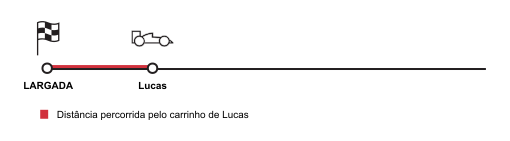
\includegraphics[width=450pt, keepaspectratio]{../../livro/media/cap2/secoes/pngs_licao_02/ativ12_fig01.png} 
\end{center}

Sabe-se que:

\begin{enumerate} [\quad a)] %s
  \item     O carrinho de Matheus só conseguiu ir metade da distância percorrida pelo carrinho de Lucas.
  \item     O carrinho de Heitor conseguiu ir até     $\frac{3}{2}$     da distância percorrida pelo carrinho de Lucas. 
  \item     O carrinho de Rafael conseguiu ir até     $\frac{4}{2}$     da distância percorrida pelo carrinho de Lucas.
  \item     O carrinho de Enzo conseguiu ir até     $\frac{5}{2}$     da distância percorrida pelo carrinho de Lucas. 
  \item     O carrinho de Nicolas conseguiu ir até     $\frac{6}{2}$     da distância percorrida pelo carrinho de Lucas. 
  \item     O carrinho de Lorenzo conseguiu ir até     $\frac{6}{4}$     da distância percorrida pelo carrinho de Lucas. 
  \item     O carrinho de Guilherme conseguiu ir até o dobro da distância percorrida pelo carrinho de Lucas.
  \item     O carrinho de Samuel conseguiu ir até     $\frac{6}{3}$     da distância percorrida pelo carrinho de Lucas. 
\end{enumerate} %s


Com estas informações, marque as posições de parada dos carrinhos de todos os amigos de Lucas no encarte que você irá receber.

\begin{center}
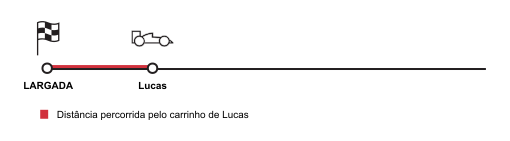
\includegraphics[width=450pt, keepaspectratio]{../../livro/media/cap2/secoes/pngs_licao_02/ativ12_fig01.png} 
\end{center}


Os carrinhos de Rafael e Samuel pararam no mesmo lugar? Explique.

\section{QUEBRANDO A CUCA }

\subsection{Atividade}

(NAEP, 1992) Pense cuidadosamente nesta questão. Escreva uma resposta completa. Você pode usar desenhos, palavras e números para explicar sua resposta. Certifique-se de mostrar todo o seu raciocínio.

José comeu $\frac{1}{2}$ de uma pizza. Ella comeu $\frac{1}{2}$ de uma outra pizza. José disse que ele comeu mais pizza do que Ella, mas Ella diz que eles comeram a mesma quantidade. Use palavras, figuras ou números para mostrar que José pode estar certo.

\subsection{Atividade}

Miguel disse para Alice que a parte pintada de vermelho na figura a seguir corresponde a $\frac{3}{5}$ da figura, pois ela está dividida em 5 partes e 3 partes estão pintadas. Você concorda com a afirmação e a justificativa de Miguel? Explique!

\begin{center}
\begin{tikzpicture}[scale=1.5]
%\fill[fill=attention,fill opacity=0.1] (0.,5.) -- (9.,5.) -- (9.,-5.) -- (0.,-5.) -- cycle;
\fill[fill=attention,fill opacity=1.0] (0.,5.) -- (0.,0.) -- (9.,0.) -- (9.,5.) -- cycle;
\fill[common, fill opacity=.3] (0,-5) rectangle (9,0);
\draw   (0.,5.)-- (9.,5.);
\draw   (9.,5.)-- (9.,-5.);
\draw   (9.,-5.)-- (0.,-5.);
\draw   (0.,-5.)-- (0.,5.);
\draw   (0.,5.)-- (0.,0.);
\draw   (0.,0.)-- (9.,0.);
\draw   (9.,0.)-- (9.,5.);
\draw   (9.,5.)-- (0.,5.);
\draw   (0.,5.)-- (9.,5.);
\draw   (9.,0.)-- (0.,0.);
\draw   (0.,0.)-- (0.,5.);
\draw   (9.,5.)-- (9.,0.);
\draw   (3.,0.)-- (3.,5.);
\draw   (6.,5.)-- (6.,0.);
\draw   (4.5,-5.)-- (4.5,0.);
\draw   (0.,-5.)-- (9.,-5.);
\draw   (9.,-5.)-- (9.,0.);
\draw   (9.,0.)-- (0.,0.);
\draw   (0.,0.)-- (0.,-5.);
% \begin{scriptsize}
% %\draw[color=ffqqqq] (4.725943121127749,2.6736730506884316) node {$pol2$};
% \end{scriptsize}
\end{tikzpicture}
\end{center}

\subsection{Atividade}

A figura a seguir tem 3 partes pintadas de vermelho e 4 partes pintadas de branco. É correto afirmar que a parte pintada de vermelho corresponde a $\frac{3}{4}$ da figura? Explique.
\begin{center}
\begin{tikzpicture}[scale=4]%[line cap=round,line join=round,>=triangle 45,x=1.0cm,y=1.0cm]
\fill[fill=attention] (0.,3.) -- (3.,3.) -- (3.,0.) -- (0.,0.) -- cycle;
\fill[common, fill opacity=.3] (3,0) rectangle (7,3);
\draw (1.,3.)-- (1.,0.);
\draw (2.,0.)-- (2.,3.);
\draw (3.,3.)-- (3.,0.);
\draw (4.,0.)-- (4.,3.);
\draw (5.,3.)-- (5.,0.);
\draw (6.,0.)-- (6.,3.);
\draw (7.,3.)-- (7.,0.);
\draw (0.,3.)-- (7.,3.);
\draw (7.,3.)-- (7.,0.);
\draw (7.,0.)-- (0.,0.);
\draw (0.,0.)-- (0.,3.);
\end{tikzpicture}
\end{center}

\subsection{Atividade}

\begin{enumerate} [\quad a)] %s
  \item     A parte em vermelho na figura a seguir representa $\frac{1}{2}$ ou $\frac{1}{4}$? 
\begin{center}
\begin{tikzpicture}[scale=1.5]
 \draw \tripinha;
\begin{scope}
 \clip \tripinha;
\draw[fill=attention] (-4,-4) rectangle (0,4);
\draw[fill=common, fill opacity=.3] (0,-4) rectangle (12,4);
\end{scope}
\end{tikzpicture} 
\end{center}
  
  \item     A parte em vermelho na figura a seguir representa     $\frac{1}{2}$     ou     $\frac{3}{2}$? 
\begin{center}
\begin{tikzpicture}[scale=1.5]
 \draw \tripa;
\begin{scope}
 \clip \tripa;
\draw[fill=attention] (-4,-4) rectangle ({4*sqrt(3)},4);
\draw[fill=common, fill opacity=.3] ({4*sqrt(3)},-4) rectangle ({12*sqrt(3)},4);
\end{scope}
\end{tikzpicture} 
\end{center}
\def \tripalonga{ (30:4) -- (90:4) -- (150:4)--(210:4)--(270:4)--(330:4) [shift={({4*sqrt(3)},0)}] --(270:4) -- (330:4) [shift={({4*sqrt(3)},0)}] --(270:4) -- (330:4)[shift={({4*sqrt(3)},0)}] --(270:4) -- (330:4) [shift={({4*sqrt(3)},0)}]--  (270:4) -- (330:4) -- (30:4) -- (90:4)--(150:4) [shift={({-4*sqrt(3)},0)}] -- (90:4) -- (150:4)[shift={({-4*sqrt(3)},0)}] -- (90:4) -- (150:4) [shift={({-4*sqrt(3)},0)}] -- (90:4) -- (150:4)--cycle;}

  \item     A parte em vermelho na figura a seguir representa     $\frac{3}{5}$     ou     $3$?
\begin{center}
\begin{tikzpicture}[scale=1.5]
 \draw \tripalonga;
\begin{scope}
 \clip \tripalonga;
  \draw[fill=attention] (-4,-4) rectangle ({10*sqrt(3)},4);
\draw[fill=common, fill opacity=.3] ({10*sqrt(3)},-4) rectangle ({20*sqrt(3)},4);  
\end{scope}
\end{tikzpicture} 
\end{center}

  \end{enumerate} %s


\subsection{Atividade}

Júlia, Davi e Laura estavam estudando a figura a seguir.
\begin{center}
\begin{tikzpicture}[scale=4]
%\fill(1.,3.) -- (6.,3.) -- (6.,0.02) -- (1.,0.) -- cycle;
\fill[attention] (1.,3.) -- (4.,3.) -- (4.,0.012) -- (1.,0.) -- cycle;
\fill[common, fill opacity=.3] (4,0) rectangle (6,3);
%\fill[line width=0.pt,color=black,fill=black,fill opacity=1.0] (4.,3.) -- (4.,0.012) -- (6.,0.04) -- (6.,3.) -- cycle;
\draw (1.,3.)-- (1.,0.);
\draw (2.,0.)-- (2.,3.);
\draw (3.,3.)-- (3.,0.);
\draw (4.,0.)-- (4.,3.);
\draw (5.,3.)-- (5.,0.);
\draw (6.,0.)-- (6.,3.);
\draw (1.,3.)-- (6.,3.);
\draw (6.,3.)-- (6.,0.02);
\draw (6.,0.02)-- (1.,0.);
\draw (1.,0.)-- (1.,3.);
\end{tikzpicture}
\end{center}
Júlia disse: ``A parte em vermelho representa $\frac{3}{5}$''. Davi retrucou: ``Não, não! A parte em vermelho representa $\frac{3}{2}$!''. Laura, então acrescentou: ``Eu acho que a parte em vermelho representa $3$!''. Quem está certo? Júlia, Davi ou Laura? Explique!

\subsection{Atividade}

Em uma pizzaria rodízio, 7 amigos comem, ao todo, 38 fatias (alternativa: simplesmente fazer o desenho das 38 fatias alinhadas, e não formando o círculo, com um triângulo ao lado de outro, caso as fatias fossem triângulos).

\begin{center}
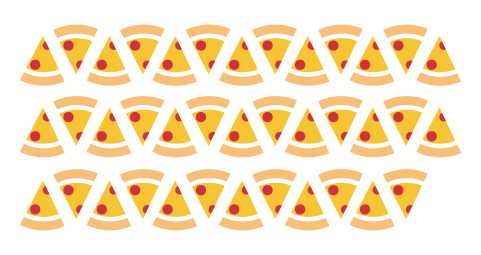
\includegraphics[width=300pt, keepaspectratio]{../../livro/media/cap2/secoes/pngs_licao_02/ativ18_fig01.png} 
\end{center}


Sabendo que nessa pizzaria cada pizza é equiparticionada em 8 partes, pergunta-se: 
\begin{enumerate} [\quad a)] %s
  \item     Quantas pizzas inteiras comeraram os 7 amigos? 
  \item     Que fração de uma pizza comeram  ao todo os amigos? 
  \item     É possível que todos os amigos tenham comido o mesmo número de fatias de pizza? Explique.
\end{enumerate} %s

